
% This LaTeX was auto-generated from an M-file by MATLAB.
% To make changes, update the M-file and republish this document.

\documentclass{article}
\usepackage{graphicx}
\usepackage{color}
\usepackage{listings}
\usepackage[framed]{mcode}
\usepackage{fullpage}
\usepackage{amsmath}
\usepackage[utf8x]{inputenc}
\usepackage{import}
\usepackage{setspace}
\usepackage{hyperref}
\definecolor{lightgray}{gray}{0.5}
\setlength{\parindent}{0pt}

\begin{document}

    
    
%\section*{}


\title{BE 521: Homework 1 \\{\normalsize Exploring Neural Signals} \\{\normalsize Spring 2021}}
\author{33 points}
\date{Due: Tuesday 2/2/2021 10 PM}
\maketitle
\textbf{Objective:} Working with the IEEG Portal to explore different Neural signals


\begin{center}
\author{Jal Mahendra Panchal}
\end{center}


\section{Seizure Activity (16 pts)}
The dataset \texttt{I521\_A0001\_D002} contains an example of human intracranial EEG (iEEG) data displaying seizure activity. It is recorded from a single channel (2 electrode contacts) implanted in the hippocampus of a patient with temporal lobe epilepsy being evaluated for surgery. In these patients, brain tissue where seizures are seen is often resected. You will do multiple comparisons with this iEEG data and the unit activity that you worked with in Homework 0 \texttt{(I521\_A0001\_D001)}. You will have to refer to that homework and/or dataset for these questions.
\begin{enumerate}
 \item Retrieve the dataset in MATLAB using the IEEGToolbox and generate a \emph{session} variable as before (No need to report the output this time). What is the sampling rate of this data? What is the maximum frequency of the signal content that we can resolve? (2 pts)

\begin{lstlisting}
%Adding workspace path
addpath(genpath('/Users/jalpanchal/git/be521'));

%create session
% dataset I521_A0001_D002.
session_sez = IEEGSession('I521_A0001_D002', 'jalpanchal', 'jal_ieeglogin.bin');

%Calculate sampling frequency in Hz
sampling_frequency_hz = session_sez.data.sampleRate

%Maximum resolvable frequency = sampling frequncy/2.
max_resolvable_freq = sampling_frequency_hz/2
\end{lstlisting}

\color{lightgray} \begin{lstlisting}IEEGSETUP: Adding 'ieeg-matlab.jar' to dynamic classpath
Warning: Objects of edu/upenn/cis/db/mefview/services/TimeSeriesDetails
class exist - not clearing java 
Warning: Objects of edu/upenn/cis/db/mefview/services/TimeSeriesInterface
class exist - not clearing java 
IEEGSETUP: Found log4j on Java classpath.
URL: https://www.ieeg.org/services
Client user: jalpanchal
Client password: ****

sampling_frequency_hz =

   200


max_resolvable_freq =

   100

\end{lstlisting} \color{black}

 \item How does the duration of this recording compare with the recording from HW0 \texttt{(I521\_A0001\_D001)}? (2 pts)

\begin{lstlisting}
duration_in_usec = session_sez.data(1).rawChannels(1).get_tsdetails.getDuration;
duration_in_sec = duration_in_usec/1e6

disp("This resording has a duration of 644.995s as compared to 10s for I521_A0001_D001")
\end{lstlisting}

\color{lightgray} \begin{lstlisting}
duration_in_sec =

  644.9950

This resording has a duration of 644.995s as compared to 10s for I521_A0001_D001
\end{lstlisting} \color{black}

 \item Using the time-series visualization functionality of the IEEG Portal, provide a screenshot of the first 500 ms of data from this recording. (2 pts)


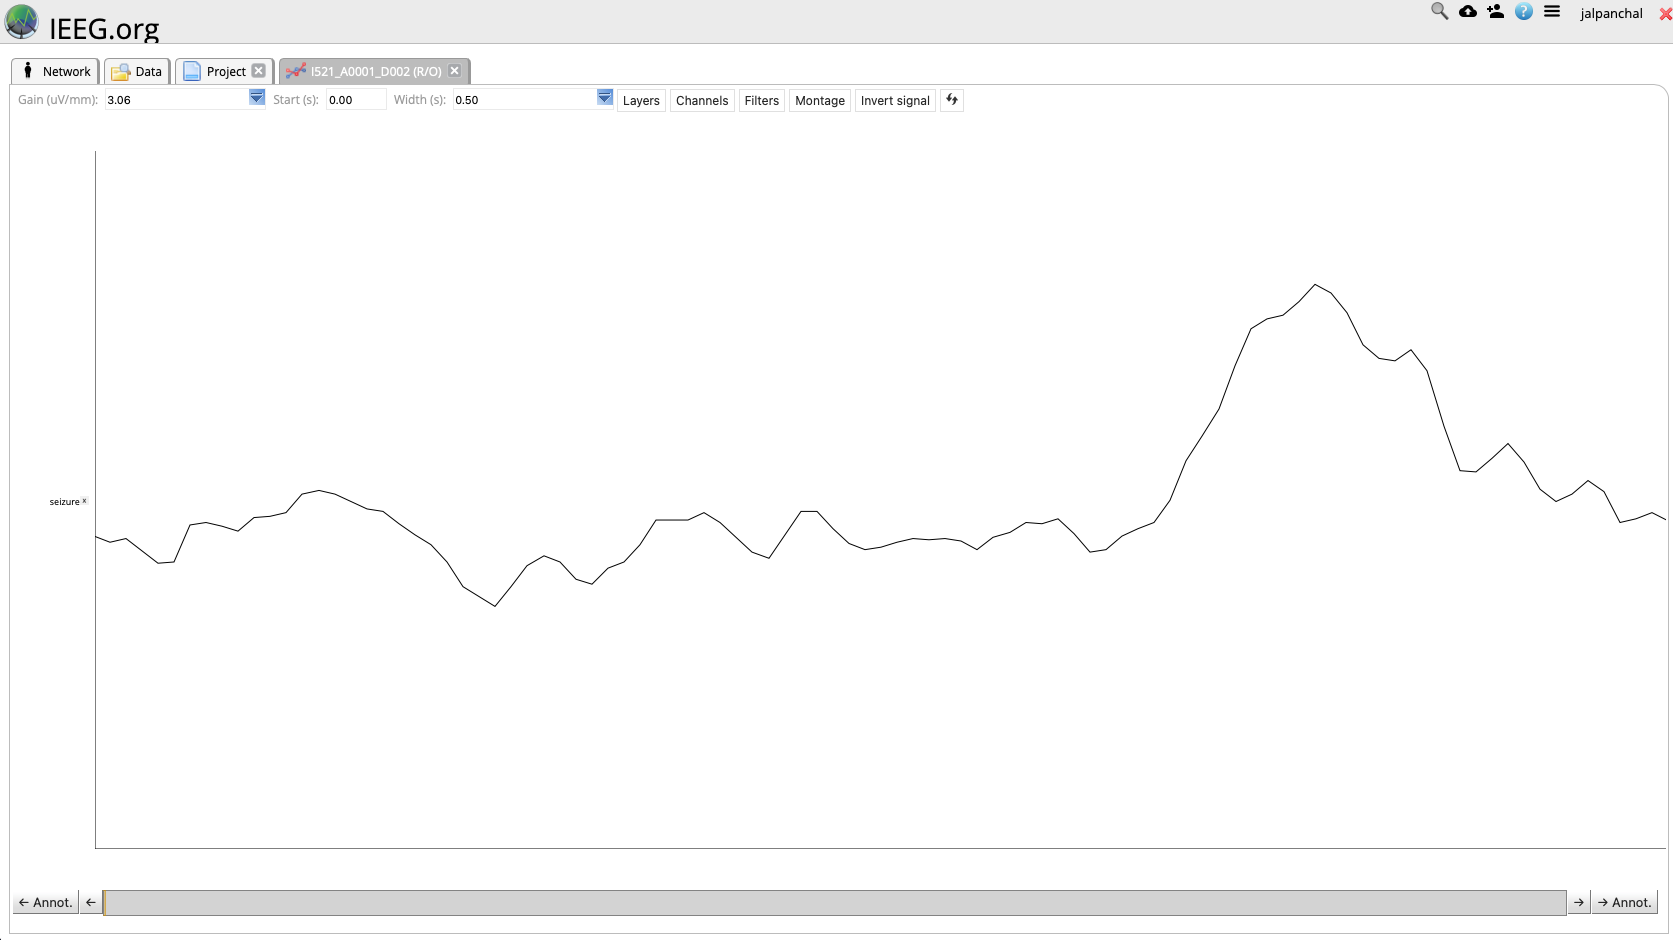
\includegraphics[scale=0.25]{screenshot_q1.3_hw1.png}\\


 \item Compare the activity in this sample with the data from HW0.  What differences do you notice in the amplitude and frequency characteristics? (2 pts)


Answer : \\
\begin{enumerate}
  \item The signal in I521\_A0001\_D002 has higher signal amplitude (Close
   to peak-peak amplitude of 4500 $\mu$V) while the I521\_A0001\_D001 signal has a
   much lower signal amplitude of about 180$\mu$V peak-peak.\\
  \item The signal in I521\_A0001\_D002 also has lower frequency
  components, with high power below 5 Hz. From the FFT, it looks like
  I521\_A0001\_D001 has a 100 Hz high-pass filter.
  \item The I521\_A0001\_D001 signal also seems to have a 3k Hz peek
  \item The I521\_A0001\_D002 signal has high amplitude, low frequency
  components from 100-200 sec as can be seen in the specogram.
\end{enumerate}

\begin{lstlisting}
%To plot frequency spectrum of each of the signals
%I521_A0001_D002

fs = sampling_frequency_hz;
len = duration_in_sec;
t = 0:1/fs:len-1/fs;
x = session_sez.data.getvalues(1, len * 1e6, 1);
y = fft(x);
n = length (x);
f = (0:n-1)*(fs/n);
power = abs(y).^2/n;

figure();
subplot(3,2,3);
plot(f(1:floor(n/2)),power(1:floor(n/2)))
title('Power Spectrum - I521\_A0001\_D002')
xlabel('Frequency (Hz)')
ylabel('Power (\mu V^2)')

%Plot of signal in time domain
subplot(3,2,1);
plot(t, x);
ylabel('Amplitude (\mu V)');
xlabel('Time (sec)');
title('Multi-unit signal - I521\_A0001\_D002');

%plotting a spectogram
subplot(3,2,5);
[p,f,t] = pspectrum(x,fs,'spectrogram');
waterfall(f,t,p');
xlabel('Frequency (Hz)')
ylabel('Time (seconds)')
zlabel('Normalized Power (\mu V^2)')
title('Spectogram - I521\_A0001\_D002');
wtf = gca;
wtf.XDir = 'reverse';
view([30 45])


%I521_A0001_D001

%Plot of Power Spectrum
session_1 = IEEGSession('I521_A0001_D001', 'jalpanchal', 'jal_ieeglogin.bin');
sampling_frequency_hz_1 = session_1.data.sampleRate;
duration_in_sec_1 = session_1.data(1).rawChannels(1).get_tsdetails.getDuration/1e6;

fs = sampling_frequency_hz_1;
len = duration_in_sec_1;
t = 0:1/fs:len-1/fs;
x = session_1.data.getvalues(1, len * 1e6, 1);
y = fft(x);
n = length (x);
f = (0:n-1)*(fs/n);
power = abs(y).^2/n;

%Plotting power spectrum
subplot(3,2,4);
plot(f(1:floor(n/2)),power(1:floor(n/2)))
title('Power Spectrum - I521\_A0001\_D001')
xlabel('Frequency (Hz)')
ylabel('Power (\mu V^2)')

%Plot of signal in time domain
subplot(3,2,2);
plot(t, x);
ylabel('Amplitude (\mu V)');
xlabel('Time (sec)');
title('Multi-unit signal - I521\_A0001\_D001');

%plotting a spectogram
subplot(3,2,6);
[p,f,t] = pspectrum(x,fs,'spectrogram');
waterfall(f,t,p');
xlabel('Frequency (Hz)')
ylabel('Time (seconds)')
zlabel('Normalized Power (\mu V^2)')
title('Spectogram - I521\_A0001\_D001');
wtf = gca;
wtf.XDir = 'reverse';
view([30 45])
\end{lstlisting}

\color{lightgray} \begin{lstlisting}IEEGSETUP: Adding 'ieeg-matlab.jar' to dynamic classpath
Warning: Objects of edu/upenn/cis/db/mefview/services/TimeSeriesDetails
class exist - not clearing java 
Warning: Objects of edu/upenn/cis/db/mefview/services/TimeSeriesInterface
class exist - not clearing java 
IEEGSETUP: Found log4j on Java classpath.
URL: https://www.ieeg.org/services
Client user: jalpanchal
Client password: ****
\end{lstlisting} \color{black}


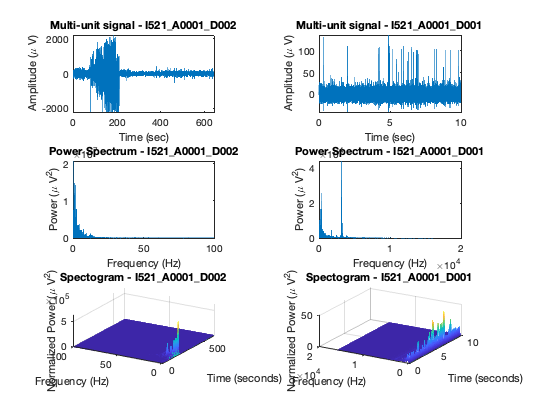
\includegraphics [width=5in]{jalp_hw1_01.png}

 \item The unit activity sample in \texttt{(I521\_A0001\_D001)} was high-pass filtered to remove low-frequency content. Assume that the seizure activity in \texttt{(I521\_A0001\_D002)} has not been high-pass filtered. Given that the power of a frequency band scales roughly as $1/f$, how might these differences in preprocessing contribute to the differences you noted in the previous question? (There is no need to get into specific calculations here. We just want general ideas.) (3 pts)


Answer : \\
\begin{enumerate}
  \item As the power of frequency band decrease with increase in
  frequences of a signal, this tells us why the power of the
  I521\_A0001\_D001 signal is lower as compared to I521\_A0001\_D002.
 \item The I521\_A0001\_D001 looks to have been filtered above 100 Hz
 while for the I521\_A0001\_D002 signal, most of the signal lies below 50
 Hz which explains the power being close to 1000 times that of
 I521\_A0001\_D001.
 \item Due to the last of a high-pass filter in I521\_A0001\_D002, this
 would also contribute to the baseline low-frequenccy base-line
 fluctuations seen in the signal as compared to the more stabel baseline
 of I521\_A0001\_D001.\\
 \end{enumerate}


 \item Two common methods of human iEEG are known as electrocorticography (ECoG) and stereoelectroencephalography (SEEG). For either of these paradigms (please indicate which you choose), find and report at least two of the following electrode characteristics: shape, material, size. Please note that exact numbers aren't required, and please cite any sources used. (3 pts)


Answer : \\
Electrocorticogram (ECoG) refers to the signal obtained from macroelectrodes
(typically 2–3 mm in diameter) placed directly on the pial surface of
cortex of epileptic patients for localization of the seizure focus \cite{lesser2010subdural}.\\
The ECoG electrodes are usually 2-3 mm in diameter, disc shaped and made
of Platinum \cite{Dubey4299}. \\


 \item What is a local field potential? How might the  characteristics of human iEEG electrodes cause them to record local field potentials as opposed to multiunit activity, which was the signal featured in HW0 as recorded from 40 micron Pt-Ir microwire electrodes? (2 pts)


Answer : \\
Local field potential (LFP) is the electric potential recorded in the
extracellular space in bain tissue \cite{Destexhe:2013}.\\ \\
For multi-unit activity, one would usually use tetrodes(set of 4
electrodes) or about 40 microns in diameter at very high frequency
(sometimes upto 30 kHz). While for LFP, the electrodes
can be larger (50 microns - 350 microns, at time even 0.5-3mm) and the
recording is done at a much lower sampling frequency, usually below 300Hz.
Having the human iEEG electrodes be larger, with lower sampling would
cause them to record LFP. \\


\end{enumerate}


\section{Evoked Potentials (17 pts)}
The data in \texttt{I521\_A0001\_D003} contains an example of a very common type of experiment and neuronal signal, the evoked potential (EP). The data show the response of the whisker barrel cortex region of rat brain to an air puff stimulation of the whiskers. The \texttt{stim} channel shows the stimulation pattern, where the falling edge of the stimulus indicates the start of the air puff, and the rising edge indicates the end. The \texttt{ep} channel shows the corresponding evoked potential.
Once again, play around with the data on the IEEG Portal, in particular paying attention to the effects of stimulation on EPs. You should observe the data with window widths of 60 secs as well as 1 sec. Again, be sure to explore the signal gain to get a more accurate picture. Finally, get a sense for how long the trials are (a constant duration) and how long the entire set of stimuli and responses are.


\begin{enumerate}
 \item Based on your observations, should we use all of the data or omit some of it? (There's no right answer, here, just make your case either way in a few sentences.) (2 pts)


Answer : \\
For the first 8 secs of data the stimulus signal seems to have a sloping
trend in the signal. Though the trigger looks to be consistently at the
second mark, this data can be ignored to keep the stimulus consistent
throughout the sample.\\ \\
The rest of the signal has a consistent stimulus signal and a response
following it so can be used for further analysis.\\
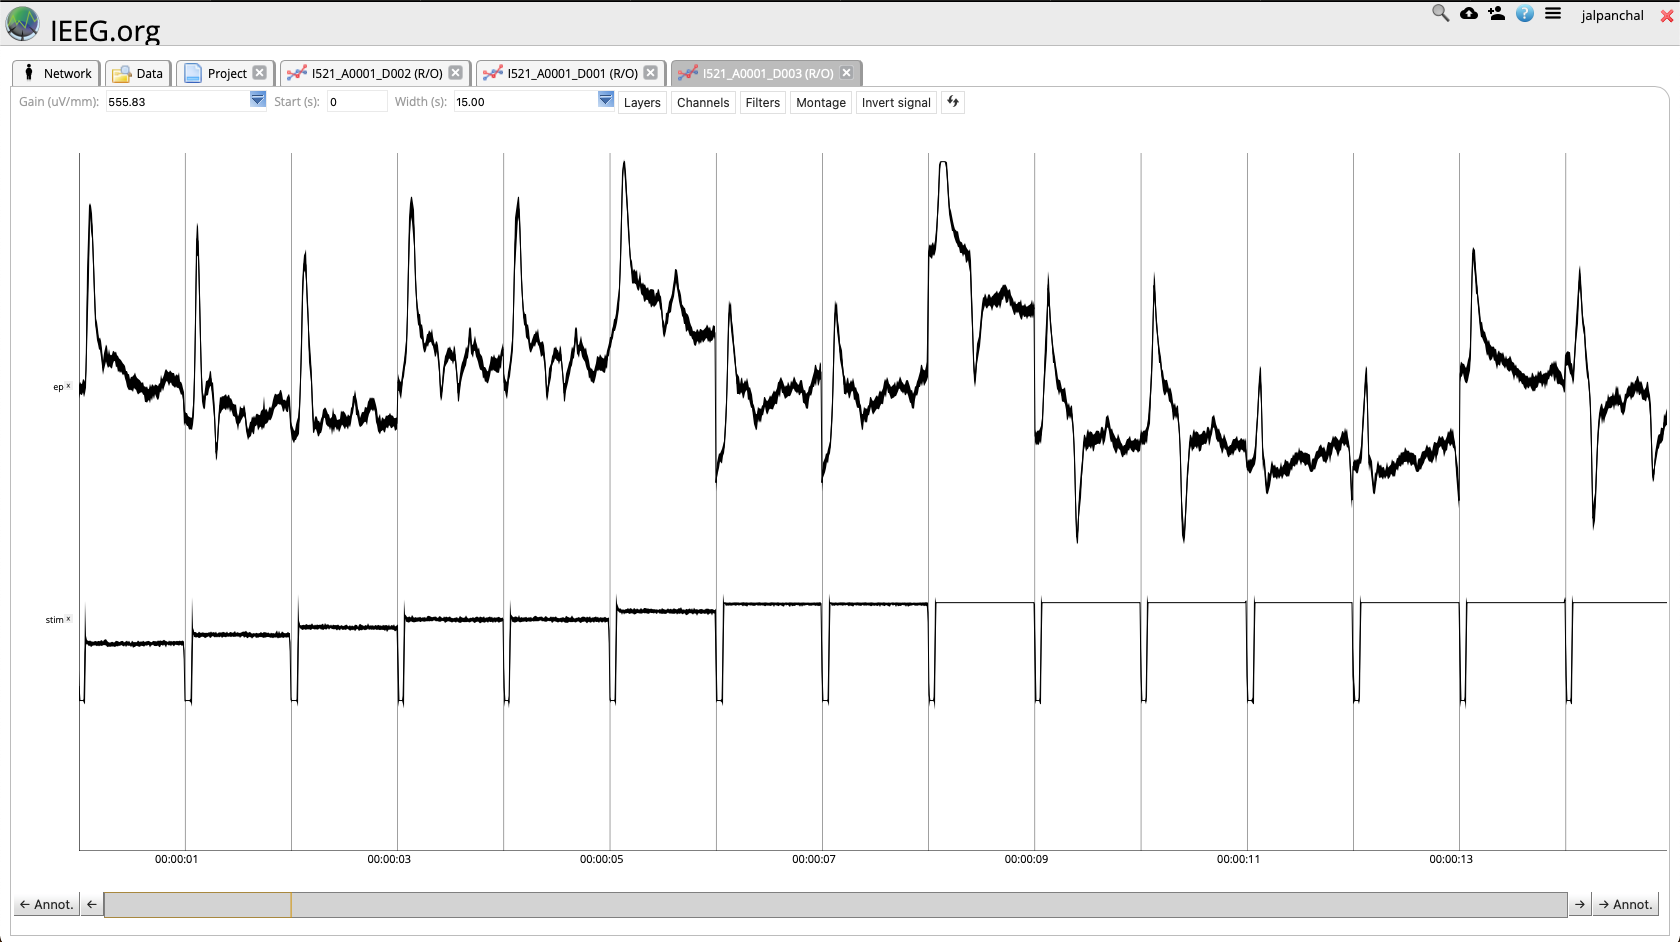
\includegraphics[scale=0.25]{screenshot_q2.1_hw1.png}\\


 \item Retrieve the \texttt{ep} and \texttt{stim} channel data in MATLAB. What is the average latency (in ms) of the peak response to the stimulus onset over all trials? (Assume stimuli occurs at exactly 1 second intervals)(3 pts)

\begin{lstlisting}
session_ep = IEEGSession('I521_A0001_D003', 'jalpanchal', 'jal_ieeglogin.bin');
sampling_frequency_hz_ep = session_ep.data.sampleRate;
duration_in_sec_ep = session_ep.data(1).rawChannels(1).get_tsdetails.getDuration/1e6;

ep_data = session_ep.data.getvalues(0, duration_in_sec_ep * 1e6, 1);
stimulus_data = session_ep.data.getvalues(0, duration_in_sec_ep * 1e6, 2);

%Making the vector size divisible by frequency to create a rectangular
%matrix of width = frequency
ep_data = [ep_data; 0];
stimulus_data = [stimulus_data; 0];

%We now have each row in the matric as a 1 sec segment of the signal
ep_data_bin = reshape(ep_data, sampling_frequency_hz_ep, [])';
stimulus_data_bin = reshape(stimulus_data, sampling_frequency_hz_ep, [])';

[ep_data_max, ep_data_max_indx] = max(ep_data_bin, [], 2);

%Calculating mean delay in response by finding the mean delay for the max
%value. Here as the data is binned at every sec, the trigger is at the
%start of every bin. So the location in the bin should directly give us the
%delay from the onset of the trigger.
disp("Average latency(in ms) of the peak response to the stimulus onset over all trials")
ep_data_peak_mean_delay_ms = (mean(ep_data_max_indx)/sampling_frequency_hz_ep)*1000


%Plot D003 with peaks
time_frame = 10 : 1/sampling_frequency_hz_ep : 15-1/sampling_frequency_hz_ep;
figure();
temp_ = ep_data_bin';
temp_ = reshape(temp_(:,10:14),[],1)';
plot(time_frame', temp_);
hold on
temp_ = [];
for n = 10:14
    temp_ = [temp_,(ep_data_bin(n,ep_data_max_indx(n)))];
end
plot((10:14) + (ep_data_max_indx(10:14)./sampling_frequency_hz_ep)', temp_, 'rx', 'MarkerSize', 10);
ylabel('Amplitude (\mu V)');
xlabel('Time (sec)');
title('Finding response peaks - I521\_A0001\_D003');
\end{lstlisting}

\color{lightgray} \begin{lstlisting}IEEGSETUP: Adding 'ieeg-matlab.jar' to dynamic classpath
Warning: Objects of edu/upenn/cis/db/mefview/services/TimeSeriesDetails
class exist - not clearing java 
Warning: Objects of edu/upenn/cis/db/mefview/services/TimeSeriesInterface
class exist - not clearing java 
IEEGSETUP: Found log4j on Java classpath.
URL: https://www.ieeg.org/services
Client user: jalpanchal
Client password: ****
Average latency(in ms) of the peak response to the stimulus onset over all trials

ep_data_peak_mean_delay_ms =

  162.1508

\end{lstlisting} \color{black}


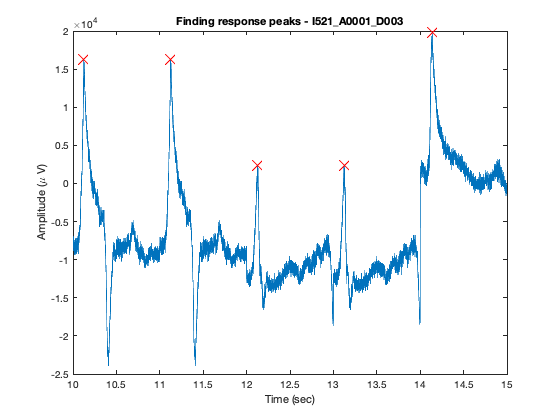
\includegraphics [width=5in]{jalp_hw1_02.png}

 \item In neuroscience, we often need to isolate a small neural signal buried under an appreciable amount of noise.  One technique to accomplish this is called the spike triggered average, sometimes called signal averaging. This technique assumes that the neural response to a repetitive stimulus is constant (or nearly so), while the noise fluctuates from trial to trial - therefore averaging the evoked response over many trials will isolate the signal and average out the noise.
 Construct a spike triggered average plot for the data in \texttt{I521\_A0001\_D003}.  Plot the average EP in red.  Using the commands \texttt{hold on} and \texttt{hold off} as well as \texttt{errorbar} and \texttt{plot}, overlay error bars at each time point on the plot to indicate the standard deviation of the responses at any given time point.  Plot the standard deviation error bars in gray (RGB value: [0.7 0.7 0.7]). Make sure to give a proper legend along with your labels. (4 pts)

\begin{lstlisting}
ep_data_mean_bin = mean(ep_data_bin,1);
stimulus_data_mean_bin = mean(stimulus_data_bin,1);

ep_stddev_timepoint = std(ep_data_bin);

time_frame = 0 : 1/sampling_frequency_hz_ep : 1-1/sampling_frequency_hz_ep;
figure();

err_bar = errorbar(time_frame, ep_data_mean_bin,ep_stddev_timepoint);
err_bar.Color  = '#B2B2B2';
legend({'Standard Deviation'}, 'FontSize', 14);
hold on
plot(time_frame', ep_data_mean_bin, 'LineWidth', 7, 'Color', 'red', 'DisplayName','Average Response');
ylabel('Amplitude (\mu V)', 'FontSize', 15);
xlabel('Time (sec)', 'FontSize', 15);
title('Avg EP Response with Standard Deviation bars - I521\_A0001\_D003', 'FontSize', 12);
\end{lstlisting}


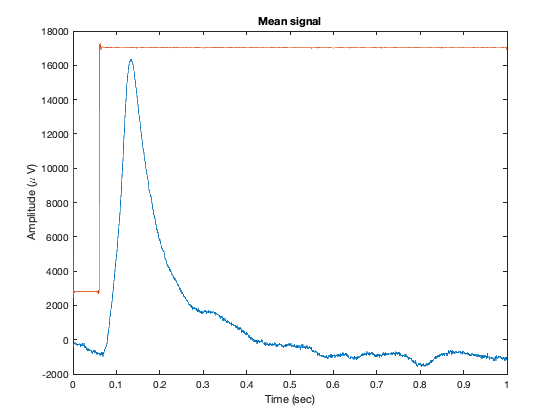
\includegraphics [width=5in]{jalp_hw1_03.png}

 \item
  \begin{enumerate}
	\item We often want to get a sense for the amplitude of the noise in a single trial. Propose a method to do this (there are a few reasonably simple methods, so no need to get too complicated). Note: do not assume that the signal averaged EP is the ``true'' signal and just subtract it from that of each trial, because whatever method you propose should be able to work on the signal from a single trial or from the average of the trials. (4 pts)

\begin{lstlisting}
%We can first begin by plotting the frequency response of the signal


fs = sampling_frequency_hz_ep;
len = duration_in_sec_ep;
t = 0:1/fs:len-1/fs;
x = session_ep.data.getvalues(1, len * 1e6, 1);
y = fft(x);
n = length (x);
f = (0:n-1)*(fs/n);
power = abs(y).^2/n;

%Plotting power spectrum
figure();
plot(f(1:floor(n/2)),power(1:floor(n/2)))
title('Power Spectrum - I521\_A0001\_D003')
xlabel('Frequency (Hz)')
ylabel('Power (\mu V^2)')
\end{lstlisting}


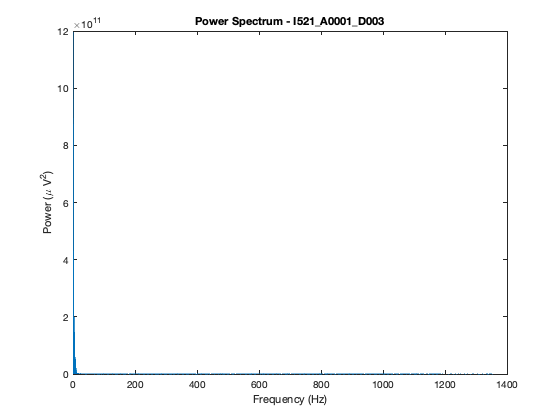
\includegraphics [width=5in]{jalp_hw1_04.png}

Let us zoom in  to the lower frequencies

\begin{lstlisting}
%Plotting power spectrum
figure();
plot(f(1:floor(n/2)),power(1:floor(n/2)))
title('Power Spectrum - I521\_A0001\_D003')
xlabel('Frequency (Hz)')
ylabel('Power (\mu V^2)')
xlim([0,50])
\end{lstlisting}


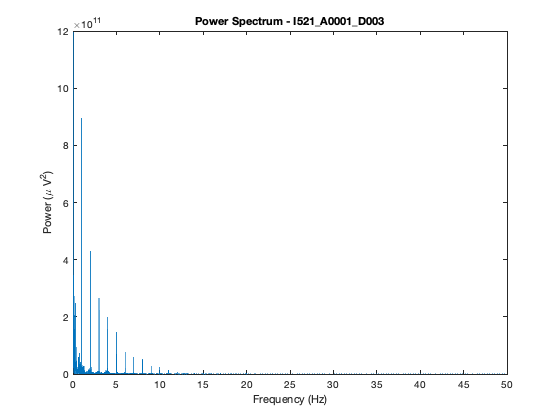
\includegraphics [width=5in]{jalp_hw1_05.png}

From the FFT of the signal we can see that the ep signal has some low
frequency niose which is causing the baseline wander and some high
frequency noise that can be seen throughout the signal. \\
to preserve the peaks, we can clean the signal by :
\begin{enumerate}
      \item Subtacting the mean of the whole segment removing any DC shift.
      \item Next we can pass the signal through a Band-pass filter to remove
  low and high frequency noise. From the FFT we can choose the values
  Lower cut-off : 1Hz and Upper cut-off : 50 Hz. \\
\end{enumerate}


	\item Show with a few of the EPs (plots and/or otherwise) that your method gives reasonable results. (1 pt)

\begin{lstlisting}
%We will remove the noise from the signal by first removing the mean from
%the signal and then using a band pass filter with a lower cut-off of 1Hz
%and a upper cut-off of 50 Hz

ep_data_mean_sub = ep_data - mean(ep_data);

%Using a bandpass filter
cut_off_freq  = [1 50];
x = ep_data_mean_sub;
fs = sampling_frequency_hz_ep;
len = size(ep_data_mean_sub,1);
t = 0:1/fs:duration_in_sec_ep+1/fs;

ep_filtered = bandpass(x, cut_off_freq, fs);
y = ep_filtered;
ep_noise = ep_data - ep_filtered;

%Selecting plotting range : 20-50s of signal
figure();
plotting_range = sampling_frequency_hz_ep*20:1:sampling_frequency_hz_ep*50;
subplot(3,1,1);
plot(t(plotting_range)',x(plotting_range));
title('Raw signal = I521\_A0001\_D003')
xlabel('Time (sec)')
ylabel('Amplitude (\mu V)')
xlim([20,50])
subplot(3,1,2);
plot(t(plotting_range)',y(plotting_range));
title('Filtered Data - I521\_A0001\_D003. Bandpass [1, 50] Hz')
xlabel('Time (sec)')
ylabel('Amplitude (\mu V)')
xlim([20,50])
subplot(3,1,3);
plot(t(plotting_range)',ep_noise(plotting_range));
title('Noise - I521\_A0001\_D003. Filer : Bandpass [1, 50] Hz')
xlabel('Time (sec)')
ylabel('Amplitude (\mu V)')
xlim([20,50])
\end{lstlisting}


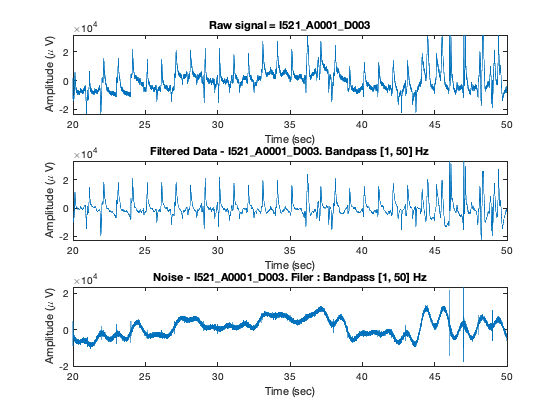
\includegraphics [width=5in]{jalp_hw1_06.png}

	\item
    \begin{enumerate}
        \item Apply your method on each individual trial and report the mean noise amplitude across all trials. (1 pt)

\begin{lstlisting}
disp("Mean of noise across all trials in \mu V")
mean_ep_noise_uV = mean(ep_noise)
\end{lstlisting}

\color{lightgray} \begin{lstlisting}Mean of noise across all trials in \mu V

mean_ep_noise_uV =

   1.0398e+03

\end{lstlisting} \color{black}

This value includes the low frequency baseline modulations, which is also
noise. \\
If we want only the the high-frequency noise, we cant pass the noise
though a high-pass filter. \\

\begin{lstlisting}
%Extracting only high-frequency noise
fs = sampling_frequency_hz_ep;
x = ep_noise;
ep_noise_highpass = highpass(x,1, fs);


%Plotting the difference after filtering
plotting_range = sampling_frequency_hz_ep*20:1:sampling_frequency_hz_ep*50;
t = 0:1/fs:duration_in_sec_ep+1/fs;
subplot(2,1,1);
plot(t(plotting_range)',ep_noise(plotting_range));
title('Noise - I521\_A0001\_D003.')
xlabel('Time (sec)')
ylabel('Amplitude (\mu V)')
xlim([20,50])
subplot(2,1,2);
plot(t(plotting_range)',ep_noise_highpass(plotting_range));
title('Filtered Noise - I521\_A0001\_D003. Filer : High-pass 1 Hz')
xlabel('Time (sec)')
ylabel('Amplitude (\mu V)')
xlim([20,50])

disp("Mean of high frequency noise in \mu V")
mean_ep_noise_highfrequency_uV = mean(ep_noise_highpass)
\end{lstlisting}

\color{lightgray} \begin{lstlisting}Mean of high frequency noise in \mu V

mean_ep_noise_highfrequency_uV =

   -0.7029

\end{lstlisting} \color{black}


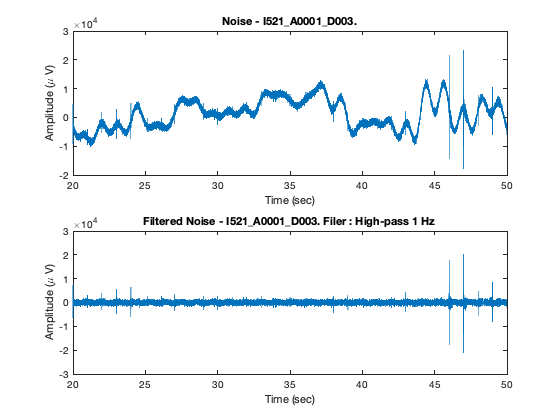
\includegraphics [width=5in]{jalp_hw1_07.png}

  \item Apply your method on the signal averaged EP and report its noise. (1 pt)

First we will substract the mean of the signal
\begin{lstlisting}
ep_mean_bin_mean_sub = ep_data_mean_bin - mean(ep_data_mean_bin);

%then we will pass the signal through a bandPass filter with cut-off [1,50]
%Hz
cut_off_freq  = [1 50];
x = ep_mean_bin_mean_sub;
fs = sampling_frequency_hz_ep;
len = size(x,2);
t = 0:1/fs:1;

ep_mean_filtered = bandpass(x, cut_off_freq, fs);
y = ep_mean_filtered;
ep_mean_noise = ep_mean_bin_mean_sub - ep_mean_filtered;

%Selecting plotting range : 20-50s of signal
figure();
plotting_range = t(1:end-1);
subplot(3,1,1);
plot(plotting_range',x);
title('Raw signal = I521\_A0001\_D003')
xlabel('Time (sec)')
ylabel('Amplitude (\mu V)')
subplot(3,1,2);
plot(plotting_range',y);
title('Filtered Data - I521\_A0001\_D003. Bandpass [1, 50] Hz')
xlabel('Time (sec)')
ylabel('Amplitude (\mu V)')
subplot(3,1,3);
plot(plotting_range',ep_mean_noise);
title('Noise - I521\_A0001\_D003. Filer : Bandpass [1, 50] Hz')
xlabel('Time (sec)')
ylabel('Amplitude (\mu V)')

disp("Mean noise level from the Average response signal is");
ep_mean_noise_level = mean(ep_mean_noise)
\end{lstlisting}

\color{lightgray} \begin{lstlisting}Mean noise level from the Average response signal is

ep_mean_noise_level =

   2.0084e+04

\end{lstlisting} \color{black}


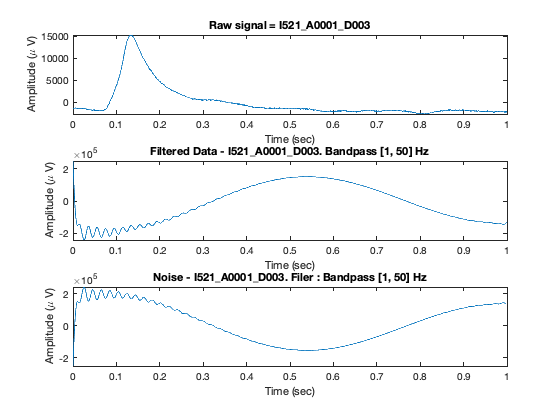
\includegraphics [width=5in]{jalp_hw1_08.png}

Here we see that due to the window of the filter function, the Average
response signal is distorted when filtered. \\
We can fix this by modifying the window or taking a longer sample
of average signal by duplicating it multiple times. \\
To keep the process consistent between the complete siganl and the
average signal, this modification will not be performed.\\


	    \item Do these two values make sense? Explain. (1 pt)


Answer :\\
\begin{enumerate}
 \item The noise value of the filtered signal with low frequency noise is
 high as expected due to basline fluctuations.
  \item With the noise filtered above 1Hz, we again see an expected noise
  signal of high frequency and a very low amplitude
\item The noise level from the filtered average response signal was quite
high due to the flaw with the filtering technique. It needs improved
windowing and finetuning to work with shorter time samples.
\end{enumerate}


    \end{enumerate}
  \end{enumerate}
\end{enumerate}
  \bibliographystyle{ieeetr}
  \bibliography{citations}




\end{document}
    
